\documentclass{ximera}

\input{../../../preamble.tex}


\definecolor{fvdnavy}{HTML}{071D43}
\definecolor{fvdcyan}{HTML}{20BFC6}
\definecolor{fvdcyanlight}{HTML}{EFFCFB}
\definecolor{fvdmagenta}{HTML}{F10D69}
\definecolor{fvdmagentalight}{HTML}{FFF1F7}
\definecolor{fvdtext}{HTML}{163044}





%=================================================
% Pedagogische omgevingen
% PDF: tcolorbox
% HTML: learning-box
%=================================================

\newenvironment{voorkennis}
{%
    \ifdefined\HCode
        \HCode{%
<section class="learning-box learning-box--prior">
<div class="learning-box__header">
<span class="learning-box__icon" aria-hidden="true"></span>
<span class="learning-box__title">Voorkennis</span>
</div>
<div class="learning-box__content">
        }%
        \begin{itemize}
    \else
       \begin{tcolorbox}[
    enhanced,
    breakable,
    colback=fvdcyanlight,
    colframe=fvdcyan,
    coltext=fvdtext,
    boxrule=0.5pt,
    leftrule=4pt,
    arc=4mm,
    outer arc=4mm,
    left=7mm,
    right=6mm,
    top=5mm,
    bottom=5mm,
    before skip=6mm,
    after skip=6mm,
    title=Voorkennis,
    coltitle=fvdcyan,
    fonttitle=\bfseries\Large,
    attach title to upper={\par\smallskip},
    boxed title style={
        empty,
        left=0mm,
        right=0mm,
        top=0mm,
        bottom=0mm
    },
    overlay={
        \draw[
            fvdcyan,
            line width=0.5pt
        ]
        ([xshift=42mm,yshift=-13mm]frame.north west)
        --
        ([xshift=-7mm,yshift=-13mm]frame.north east);
    }
]
        \begin{itemize}
    \fi
}
{%
    \end{itemize}
    \ifdefined\HCode
        \HCode{%
</div>
</section>
        }%
    \else
        \end{tcolorbox}
    \fi
}


\newenvironment{leerdoelen}
{%
    \ifdefined\HCode
        \HCode{%
<section class="learning-box learning-box--goals">
<div class="learning-box__header">
<span class="learning-box__icon" aria-hidden="true"></span>
<span class="learning-box__title">Leerdoelen</span>
</div>
<div class="learning-box__content">
        }%
        \begin{itemize}
    \else
\begin{tcolorbox}[
    enhanced,
    breakable,
    colback=fvdmagentalight,
    colframe=fvdmagenta,
    coltext=fvdtext,
    boxrule=0.5pt,
    leftrule=4pt,
    arc=4mm,
    outer arc=4mm,
    left=7mm,
    right=6mm,
    top=5mm,
    bottom=5mm,
    before skip=6mm,
    after skip=6mm,
    title=Leerdoelen,
    coltitle=fvdmagenta,
    fonttitle=\bfseries\Large,
    attach title to upper={\par\smallskip},
    boxed title style={
        empty,
        left=0mm,
        right=0mm,
        top=0mm,
        bottom=0mm
    },
    overlay={
        \draw[
            fvdmagenta,
            line width=0.5pt
        ]
        ([xshift=42mm,yshift=-13mm]frame.north west)
        --
        ([xshift=-7mm,yshift=-13mm]frame.north east);
    }
]
        \begin{itemize}
    \fi
}
{%
    \end{itemize}
    \ifdefined\HCode
        \HCode{%
</div>
</section>
        }%
    \else
        \end{tcolorbox}
    \fi
}



\title{Oppervlakte als som van kleine stukjes}
\author{Ingmar Herreman}

\begin{document}

% FVD_CHAPTER_DATA_START
% Automatisch gegenereerd uit index.tex.
% Niet handmatig aanpassen.
\fvdchapterdata{2}{Van oppervlakte naar integraal}{1}
% FVD_CHAPTER_DATA_END


% ============================================================
% ABSTRACT
% ============================================================

\begin{abstract}
Een oppervlakte onder een grafiek is meer dan een meetkundige figuur.
Ze kan ook de totale bijdrage van een veranderende grootheid over een
interval beschrijven.

In dit hoofdstuk onderzoeken we hoe oppervlakten boven en onder de
\(x\)-as samen één \textbf{georiënteerde oppervlakte} vormen. We leren
grafieken opdelen in gekende vlakke figuren, letten op het teken van
elke bijdrage en gebruiken eenheden om de betekenis van een oppervlakte
te achterhalen.

Aan het einde botsen we op een nieuw probleem: wat doen we wanneer de
grafiek gekromd is en de oppervlakte niet meer exact met rechthoeken,
driehoeken of trapezia kan worden berekend? Dat probleem leidt in het
volgende hoofdstuk naar de bepaalde integraal.
\end{abstract}

\maketitle


% ============================================================
% VOORKENNIS EN LEERDOELEN
% ============================================================

\begin{voorkennis}
  \item Je kan de oppervlakte van een rechthoek, driehoek en trapezium berekenen.
  \item Je kan een grafiek aflezen.
  \item Je kan nulpunten en het teken van een functie uit een grafiek bepalen.
  \item Je kan werken met grootheden en eenheden.
\end{voorkennis}

\begin{leerdoelen}
  \item Je kan een gebied tussen een grafiek en de \(x\)-as opdelen in eenvoudige vlakke figuren.
  \item Je kan de gewone oppervlakte van zo'n gebied berekenen.
  \item Je kan positieve en negatieve bijdragen in een grafiek herkennen.
  \item Je kan een georiënteerde oppervlakte berekenen en interpreteren.
  \item Je kan het verschil uitleggen tussen gewone en georiënteerde oppervlakte.
  \item Je kan uit de grootheden en eenheden op de assen afleiden welke grootheid een oppervlakte onder een grafiek kan voorstellen.
  \item Je kan in een eenvoudige context uitleggen wat positieve en negatieve bijdragen betekenen.
  \item Je kan aangeven waarom gekende meetkundige oppervlakteformules niet volstaan voor een algemene gekromde grafiek.
\end{leerdoelen}


% ============================================================
% 1. OPPERVLAKTE ONDER EEN GRAFIEK
% ============================================================

\FVDsection{Oppervlakte onder een grafiek}

We kennen oppervlakte vooral uit de meetkunde. Voor een rechthoek met
breedte \(b\) en hoogte \(h\) geldt

\[
S=b\cdot h.
\]

Voor een driehoek geldt

\[
S=\frac12 bh.
\]

Ook wanneer zulke figuren onder een grafiek liggen, kunnen we deze
gekende formules gebruiken.

\begin{voorbeeld}[Een gebied opdelen]

Beschouw de onderstaande grafiek.

\begin{center}
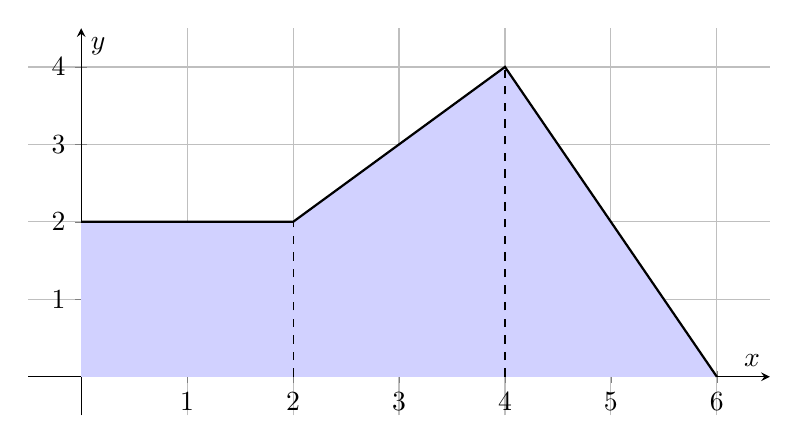
\begin{tikzpicture}
\begin{axis}[
    axis lines=middle,
    xmin=-0.5, xmax=6.5,
    ymin=-0.5, ymax=4.5,
    xlabel={$x$},
    ylabel={$y$},
    xtick={0,1,2,3,4,5,6},
    ytick={0,1,2,3,4},
    grid=both,
    width=11cm,
    height=6.5cm
]
    \draw[fill=blue!18,draw=none]
        (axis cs:0,0)--(axis cs:0,2)--(axis cs:2,2)--(axis cs:4,4)--(axis cs:6,0)--cycle;

    \addplot[black,thick] coordinates {(0,2) (2,2) (4,4) (6,0)};
    \draw[dashed] (axis cs:2,0)--(axis cs:2,2);
    \draw[dashed] (axis cs:4,0)--(axis cs:4,4);
\end{axis}
\end{tikzpicture}
\end{center}

Het gebied kan bijvoorbeeld worden opgesplitst in een rechthoek en
twee trapezia. Omdat elk deel boven de \(x\)-as ligt, kunnen we de
gewone oppervlakten optellen.

Het belangrijke idee is niet welke opdeling je kiest, maar wel dat
\textbf{het totale gebied kan worden opgebouwd uit kleinere bijdragen}.
\end{voorbeeld}

\begin{opmerking}
Een slimme opdeling maakt een oppervlakteberekening vaak eenvoudiger.
Dezelfde figuur kan op verschillende correcte manieren worden
opgedeeld.
\end{opmerking}


% ============================================================
% 2. WAT GEBEURT ER ONDER DE X-AS?
% ============================================================

\FVDsection{Boven en onder de \(x\)-as}

Beschouw nu een grafiek die zowel boven als onder de \(x\)-as ligt.

\begin{center}
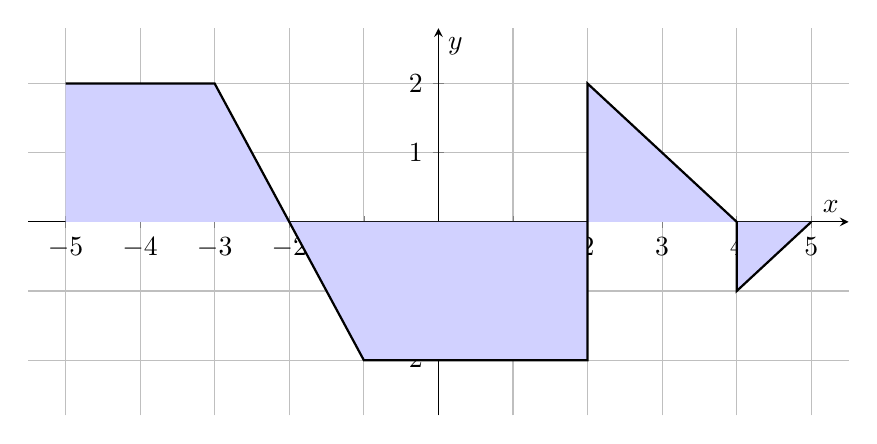
\begin{tikzpicture}
\begin{axis}[
    axis lines=middle,
    xmin=-5.5, xmax=5.5,
    ymin=-2.8, ymax=2.8,
    xlabel={$x$},
    ylabel={$y$},
    xtick={-5,-4,...,5},
    ytick={-2,-1,0,1,2},
    grid=both,
    width=12cm,
    height=6.5cm
]
    \draw[fill=blue!18,draw=none]
        (axis cs:-5,0)--(axis cs:-5,2)--(axis cs:-3,2)--(axis cs:-2,0)--cycle;
    \draw[fill=blue!18,draw=none]
        (axis cs:-2,0)--(axis cs:-1,-2)--(axis cs:2,-2)--(axis cs:2,0)--cycle;
    \draw[fill=blue!18,draw=none]
        (axis cs:2,0)--(axis cs:2,2)--(axis cs:4,0)--cycle;
    \draw[fill=blue!18,draw=none]
        (axis cs:4,0)--(axis cs:5,0)--(axis cs:4,-1)--cycle;

    \addplot[black,thick] coordinates {
        (-5,2) (-3,2) (-2,0) (-1,-2) (2,-2) (2,2) (4,0) (4,-1) (5,0)
    };
\end{axis}
\end{tikzpicture}
\end{center}

Als we naar de \emph{gewone meetkundige oppervlakte} kijken, is elk
deel positief. Een oppervlakte van bijvoorbeeld \(3\) vierkante
eenheden blijft \(3\), ongeacht of het gebied boven of onder de
\(x\)-as ligt.

Toch is het in veel wiskundige situaties nuttig om gebieden onder de
\(x\)-as een negatief teken te geven. Daardoor kunnen verschillende
bijdragen elkaar versterken of gedeeltelijk opheffen.

\begin{definitie}
De \textbf{georiënteerde oppervlakte} tussen de grafiek van een functie
en de \(x\)-as wordt bepaald door aan elk deel een teken toe te kennen:

\begin{itemize}
    \item een gebied \textbf{boven de \(x\)-as} levert een positieve bijdrage;
    \item een gebied \textbf{onder de \(x\)-as} levert een negatieve bijdrage.
\end{itemize}

De georiënteerde oppervlakte is de som van al deze positieve en
negatieve bijdragen.
\end{definitie}


% ============================================================
% 3. GEWONE EN GEORIENTEERDE OPPERVLAKTE
% ============================================================

\FVDsection{Gewone en georiënteerde oppervlakte}

Stel dat een grafiek een positieve oppervlakte \(S_+\) en een
oppervlakte \(S_-\) onder de \(x\)-as begrenst. Hier stellen
\(S_+\) en \(S_-\) de \emph{gewone}, dus positieve, oppervlakten van de
betrokken gebieden voor.

Voor de totale gewone oppervlakte geldt

\[
S_{\mathrm{opp}}=S_+ + S_-.
\]

Voor de georiënteerde oppervlakte geldt daarentegen

\[
S_{\mathrm{geo}}=S_+ - S_-.
\]

\begin{voorbeeld}[Zelfde gebieden, andere vraag]

Veronderstel dat

\[
S_+=9
\qquad\text{en}\qquad
S_-=5.
\]

Dan is de totale gewone oppervlakte

\[
S_{\mathrm{opp}}=9+5=14,
\]

terwijl de georiënteerde oppervlakte gelijk is aan

\[
S_{\mathrm{geo}}=9-5=4.
\]

De twee antwoorden horen dus bij twee verschillende vragen.
\end{voorbeeld}

\begin{eigenschap}
Een georiënteerde oppervlakte kan positief, negatief of nul zijn.

In het bijzonder kan

\[
S_{\mathrm{geo}}=0
\]

terwijl er toch verschillende gebieden tussen de grafiek en de
\(x\)-as liggen. Dat gebeurt wanneer de totale positieve en negatieve
bijdragen even groot zijn.
\end{eigenschap}

\begin{voorbeeld}[Een totale bijdrage van nul]

Als

\[
S_+=6
\qquad\text{en}\qquad
S_-=6,
\]

dan

\[
S_{\mathrm{geo}}=6-6=0.
\]

De gewone totale oppervlakte is echter

\[
S_{\mathrm{opp}}=6+6=12.
\]

Een georiënteerde oppervlakte van nul betekent dus niet dat er
``geen oppervlakte'' is. Het betekent dat de positieve en negatieve
bijdragen elkaar precies compenseren.
\end{voorbeeld}


% ============================================================
% 4. OPPERVLAKTE ALS TOTALE VERANDERING
% ============================================================

\FVDsection{Oppervlakte als totale verandering}

Tot nu toe hebben we oppervlakte vooral bekeken als een meetkundige
grootheid. Onder een grafiek kan een oppervlakte echter ook een
\textbf{verandering van een andere grootheid} voorstellen.

Stel dat een grootheid \(r\) aangeeft hoeveel er per eenheid wordt
toegevoegd of weggenomen.

Als \(r\) gedurende een interval constant is, dan geldt

\[
\boxed{
\text{totale verandering}
=
\text{verandering per eenheid}
\cdot
\text{lengte van het interval}
}
\]

Meetkundig is dit precies de oppervlakte van een rechthoek.

\begin{center}
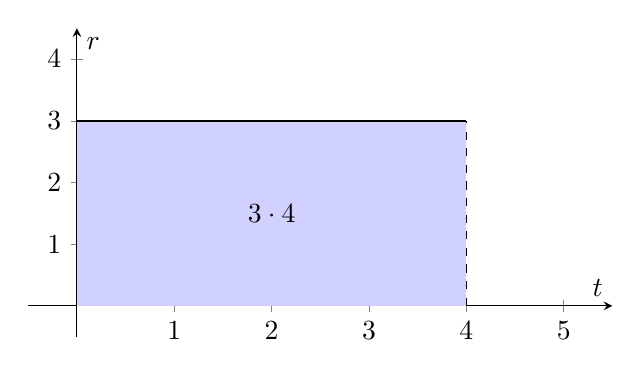
\begin{tikzpicture}
\begin{axis}[
    axis lines=middle,
    xmin=-0.5, xmax=5.5,
    ymin=-0.5, ymax=4.5,
    xlabel={$t$},
    ylabel={$r$},
    xtick={0,1,2,3,4,5},
    ytick={0,1,2,3,4},
    width=9cm,
    height=5.5cm
]
    \draw[fill=blue!18,draw=none]
        (axis cs:0,0) rectangle (axis cs:4,3);

    \addplot[black,thick,domain=0:4] {3};

    \draw[dashed] (axis cs:4,0)--(axis cs:4,3);

    \node at (axis cs:2,1.5) {$3\cdot4$};
\end{axis}
\end{tikzpicture}
\end{center}

De oppervlakte onder een grafiek hoeft dus niet noodzakelijk een
meetkundige oppervlakte voor te stellen. Ze kan ook aangeven hoeveel
een grootheid in totaal veranderd is.

\begin{opmerking}
De eenheid van de oppervlakte onder een grafiek wordt bepaald door de
eenheden op beide assen met elkaar te vermenigvuldigen.

De uitkomst hoeft dus niet bijvoorbeeld \(\mathrm{m^2}\) te zijn.
\end{opmerking}


% ============================================================
% VOORBEELD 1: DEBIET
% ============================================================

\begin{voorbeeld}[Een tank vullen en leegmaken]

Een tank bevat aanvankelijk \(15\) liter vloeistof. Een meter registreert
het debiet \(d\) in \(\mathrm{L/min}\).

Een positief debiet betekent dat vloeistof wordt toegevoegd; een
negatief debiet betekent dat vloeistof uit de tank verdwijnt.

\begin{center}
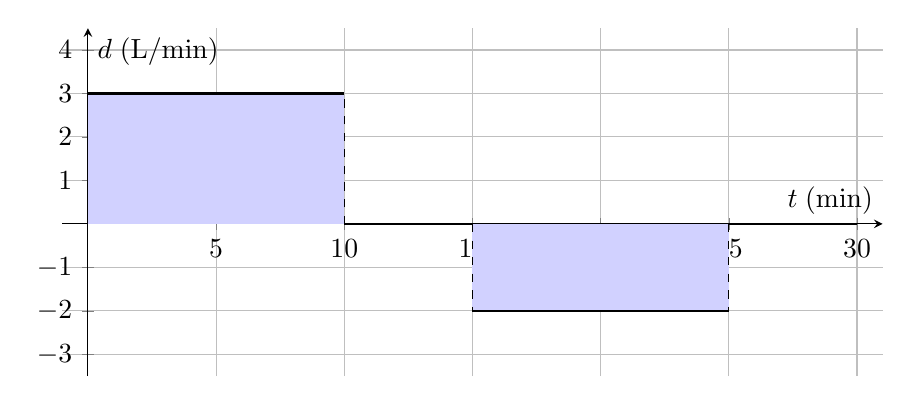
\begin{tikzpicture}
\begin{axis}[
    axis lines=middle,
    xmin=-1, xmax=31,
    ymin=-3.5, ymax=4.5,
    xlabel={$t\;(\mathrm{min})$},
    ylabel={$d\;(\mathrm{L/min})$},
    xtick={0,5,10,15,20,25,30},
    ytick={-3,-2,-1,0,1,2,3,4},
    grid=both,
    width=12cm,
    height=6cm
]
    \draw[fill=blue!18,draw=none]
        (axis cs:0,0)--(axis cs:0,3)--(axis cs:10,3)--(axis cs:10,0)--cycle;

    \draw[fill=blue!18,draw=none]
        (axis cs:15,0)--(axis cs:15,-2)--(axis cs:25,-2)--(axis cs:25,0)--cycle;

    \addplot[black,thick] coordinates {(0,3) (10,3)};
    \addplot[black,thick] coordinates {(10,0) (15,0)};
    \addplot[black,thick] coordinates {(15,-2) (25,-2)};
    \addplot[black,thick] coordinates {(25,0) (30,0)};

    \draw[dashed] (axis cs:10,0)--(axis cs:10,3);
    \draw[dashed] (axis cs:15,0)--(axis cs:15,-2);
    \draw[dashed] (axis cs:25,0)--(axis cs:25,-2);
\end{axis}
\end{tikzpicture}
\end{center}

Tijdens de eerste \(10\) minuten is het debiet constant en gelijk aan

\[
3\ \mathrm{L/min}.
\]

De hoeveelheid vloeistof die wordt toegevoegd is

\[
3\cdot10=30\ \mathrm L.
\]

Dat is precies de oppervlakte van het rechthoekige gebied boven de
tijdas.

Van \(t=10\) tot \(t=15\) is het debiet nul. In die periode verandert
het volume dus niet.

Van \(t=15\) tot \(t=25\) is het debiet

\[
-2\ \mathrm{L/min}.
\]

De bijdrage in die periode is

\[
(-2)\cdot10=-20\ \mathrm L.
\]

Het minteken betekent dat er vloeistof uit de tank verdwijnt.

De totale verandering van het volume over de eerste \(25\) minuten is

\[
30-20=10\ \mathrm L.
\]

Omdat de tank aanvankelijk \(15\) liter bevatte, is het volume na
\(25\) minuten

\[
15+10=25\ \mathrm L.
\]

Merk ook op dat de eenheden kloppen:

\[
\frac{\mathrm L}{\mathrm{min}}
\cdot
\mathrm{min}
=
\mathrm L.
\]

De oppervlakte onder de debietgrafiek stelt hier dus een
\textbf{verandering van volume} voor.

\end{voorbeeld}


% ============================================================
% VOORBEELD 2: BEWEGING
% ============================================================

\begin{voorbeeld}[Een loper keert terug]

Een loper beweegt gedurende een half uur met een constante snelheid van

\[
10\ \mathrm{km/h}.
\]

Daarna keert hij om en beweegt hij gedurende een half uur met snelheid

\[
-6\ \mathrm{km/h}.
\]

Het minteken geeft aan dat hij in de tegengestelde richting beweegt.

\begin{center}
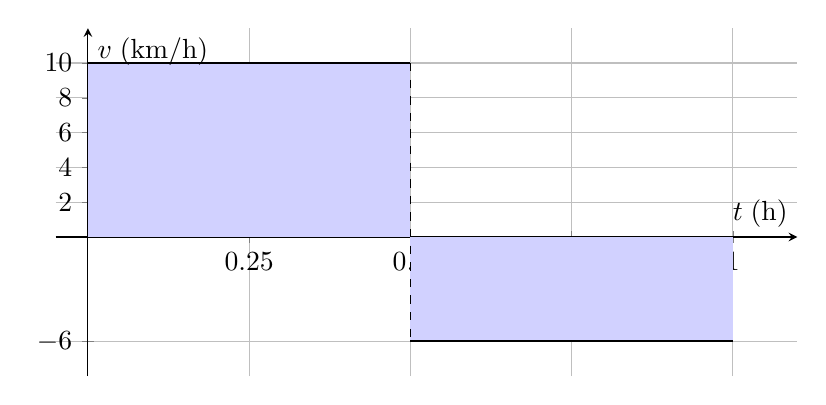
\begin{tikzpicture}
\begin{axis}[
    axis lines=middle,
    xmin=-0.05, xmax=1.1,
    ymin=-8, ymax=12,
    xlabel={$t\;(\mathrm h)$},
    ylabel={$v\;(\mathrm{km/h})$},
    xtick={0,0.25,0.5,0.75,1},
    ytick={-6,0,2,4,6,8,10},
    grid=both,
    width=11cm,
    height=6cm
]
    \draw[fill=blue!18,draw=none]
        (axis cs:0,0) rectangle (axis cs:0.5,10);

    \draw[fill=blue!18,draw=none]
        (axis cs:0.5,0) rectangle (axis cs:1,-6);

    \addplot[black,thick] coordinates {(0,10) (0.5,10)};
    \addplot[black,thick] coordinates {(0.5,-6) (1,-6)};

    \draw[dashed] (axis cs:0.5,10)--(axis cs:0.5,-6);
\end{axis}
\end{tikzpicture}
\end{center}

Tijdens het eerste half uur is de bijdrage

\[
10\cdot0.5=5\ \mathrm{km}.
\]

Tijdens het tweede half uur is de bijdrage

\[
(-6)\cdot0.5=-3\ \mathrm{km}.
\]

De totale georiënteerde bijdrage is dus

\[
5-3=2\ \mathrm{km}.
\]

De loper bevindt zich na één uur \(2\) km in de positieve richting
ten opzichte van zijn vertrekpunt.

De totaal afgelegde weg is echter

\[
5+3=8\ \mathrm{km}.
\]

Ook hier vertellen de eenheden wat de oppervlakte betekent:

\[
\frac{\mathrm{km}}{\mathrm h}
\cdot
\mathrm h
=
\mathrm{km}.
\]

De oppervlakte onder een snelheid-tijdgrafiek kan dus een
\textbf{verplaatsing} voorstellen.

\begin{opmerking}
In een snelheid-tijdgrafiek moet je onderscheid maken tussen:

\begin{itemize}
    \item de \textbf{verplaatsing}: positieve en negatieve bijdragen
    worden met hun teken opgeteld;

    \item de \textbf{afgelegde weg}: alle afgelegde stukken worden
    positief opgeteld.
\end{itemize}
\end{opmerking}

\end{voorbeeld}


% ============================================================
% CENTRAAL IDEE
% ============================================================

\begin{opmerking}
In beide voorbeelden gebeurt hetzelfde:

\[
\boxed{
\text{totale verandering}
=
\text{som van positieve en negatieve bijdragen}
}
\]

De oppervlakte onder een grafiek kan dus een manier zijn om zulke
bijdragen over een interval samen te nemen.

In het volgende hoofdstuk zullen we onderzoeken hoe dit idee ook werkt
wanneer de grafiek niet uit horizontale lijnstukken bestaat.
\end{opmerking}


% ============================================================
% 7. REDENEREN MET EEN GRAFIEK
% ============================================================

\FVDsection{Redeneren zonder meteen te rekenen}

Een grafiek kan vaak al veel informatie geven voordat we een oppervlakte
exact berekenen.

Als een functie \(f\) op een interval boven de \(x\)-as ligt, dan is de
georiënteerde bijdrage op dat interval positief.

Als \(f\) onder de \(x\)-as ligt, dan is die bijdrage negatief.

Daarom kunnen we soms het teken van de totale georiënteerde oppervlakte
voorspellen door de verschillende gebieden met elkaar te vergelijken.

\begin{voorbeeld}[Welke bijdrage overheerst?]

    Veronderstel dat een grafiek op \([a,b]\) eerst boven en daarna onder de
    \(x\)-as ligt.
    
    \begin{center}
    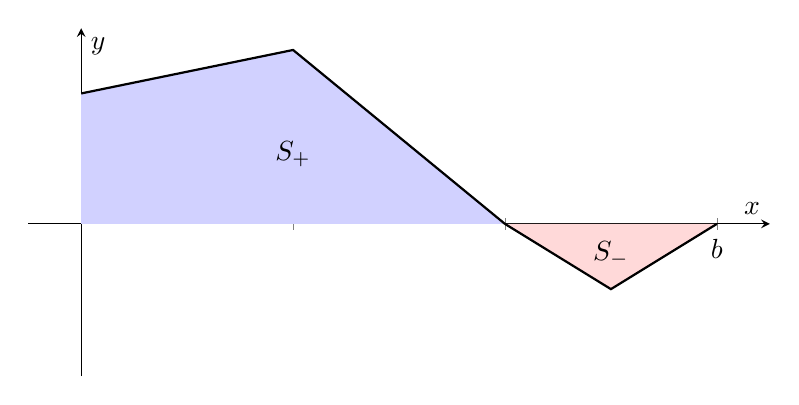
\begin{tikzpicture}
    \begin{axis}[
        axis lines=middle,
        xmin=-0.5, xmax=6.5,
        ymin=-3.5, ymax=4.5,
        xlabel={$x$},
        ylabel={$y$},
        xtick={0,2,4,6},
        xticklabels={$a$,,, $b$},
        ytick=\empty,
        width=11cm,
        height=6cm
    ]
    
        % positieve gebied
        \draw[fill=blue!18,draw=none]
            (axis cs:0,0)
            -- (axis cs:0,3)
            -- (axis cs:2,4)
            -- (axis cs:4,0)
            -- cycle;
    
        % negatieve gebied
        \draw[fill=red!15,draw=none]
            (axis cs:4,0)
            -- (axis cs:5,-1.5)
            -- (axis cs:6,0)
            -- cycle;
    
        % grafiek
        \addplot[
            black,
            thick
        ] coordinates {
            (0,3)
            (2,4)
            (4,0)
            (5,-1.5)
            (6,0)
        };
    
        % labels
        \node at (axis cs:2,1.6) {$S_+$};
        \node at (axis cs:5,-0.7) {$S_-$};
    
    \end{axis}
    \end{tikzpicture}
    \end{center}
    
    In deze figuur is het positieve gebied duidelijk groter dan het negatieve
    gebied. We verwachten dus
    
    \[
    S_{\mathrm{geo}}>0.
    \]
    
    Als beide gebieden even groot zijn, dan
    
    \[
    S_{\mathrm{geo}}=0.
    \]
    
    Als het gebied onder de as groter is, dan
    
    \[
    S_{\mathrm{geo}}<0.
    \]
    
    Voor deze conclusie hoeven we niet noodzakelijk elk gebied afzonderlijk
    exact te berekenen.
    
    \end{voorbeeld}


% ============================================================
% 8. DE GRENS VAN ONZE HUIDIGE METHODE
% ============================================================

\FVDsection{Wat als de grafiek gekromd is?}

Tot nu toe kozen we grafieken waarvoor de gebieden konden worden
opgedeeld in rechthoeken, driehoeken en trapezia.

Beschouw nu \(
f(x)=x^2+1\)

op het interval \([0,3]\).

\begin{center}
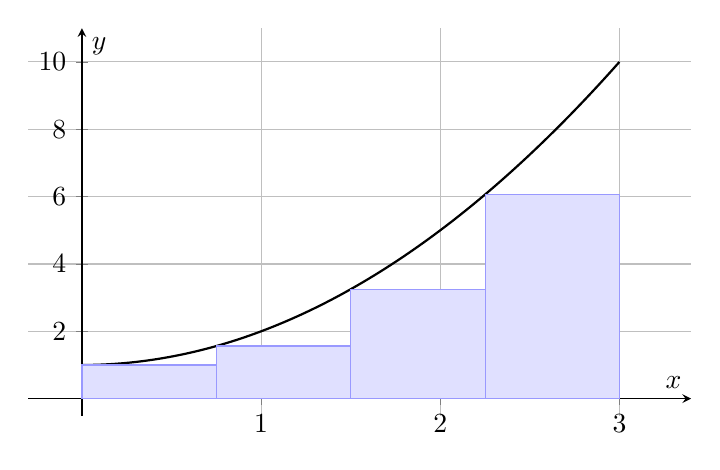
\begin{tikzpicture}
\begin{axis}[
    axis lines=middle,
    xmin=-0.3, xmax=3.4,
    ymin=-0.5, ymax=11,
    xlabel={$x$},
    ylabel={$y$},
    xtick={0,1,2,3},
    ytick={0,2,4,6,8,10},
    grid=both,
    width=10cm,
    height=6.5cm
]
    \addplot[black,thick,domain=0:3,samples=100] {x^2+1};

    \draw[fill=blue!12,draw=blue!40]
        (axis cs:0,0) rectangle (axis cs:0.75,1);
    \draw[fill=blue!12,draw=blue!40]
        (axis cs:0.75,0) rectangle (axis cs:1.5,1.5625);
    \draw[fill=blue!12,draw=blue!40]
        (axis cs:1.5,0) rectangle (axis cs:2.25,3.25);
    \draw[fill=blue!12,draw=blue!40]
        (axis cs:2.25,0) rectangle (axis cs:3,6.0625);
\end{axis}
\end{tikzpicture}
\end{center}

Het gebied onder deze grafiek is niet opgebouwd uit een eindig aantal
rechthoeken, driehoeken of trapezia.

We kunnen de oppervlakte wel \emph{benaderen} door rechthoeken te
gebruiken.

Met weinig brede rechthoeken is de benadering nog ruw. Als we het
interval in meer stukken verdelen, worden de rechthoeken smaller en
kan de benadering nauwkeuriger worden.

Dit leidt tot een nieuwe vraag:

\begin{center}
\textbf{Wat gebeurt er als we steeds meer en steeds smallere
rechthoeken gebruiken?}
\end{center}

Het antwoord op die vraag brengt ons in het volgende hoofdstuk bij
\textbf{sommen, limieten en de bepaalde integraal}.

\end{document}